%----------------------------------------------------------------------------
\appendix
%----------------------------------------------------------------------------
%\chapter*{\fuggelek}\addcontentsline{toc}{chapter}{\fuggelek}
%\setcounter{chapter}{\appendixnumber}
%\setcounter{equation}{0} % a fofejezet-szamlalo az angol ABC 6. betuje (F) lesz
%\numberwithin{equation}{section}
%\numberwithin{figure}{section}
%\numberwithin{lstlisting}{section}
%\numberwithin{tabular}{section}



%----------------------------------------------------------------------------
\chapter{LTL Expressions}
%----------------------------------------------------------------------------

%----------------------------------------------------------------------------
\section{The Syntax of the LTL Expressions}
%----------------------------------------------------------------------------
\begin{lstlisting} [language=tex,caption=Full syntax of the LTL expressions using the EBNF notation \cite{EBNFStandard},label=lst_ltlfullsyntax]
	LTLExpression = ArrowExpression;
	ArrowExpression = (OrExpression '->' ArrowExpression) |
	                    (OrExpression '<->' ArrowExpression) |
	                     OrExpression;
	OrExpression = (OrExpression '|' AndExpression) |
	                  AndExpression;
	AndExpression = (AndExpression '&' UntilExpression) |
	                   UntilExpression;
	UntilExpression = (FutureGloballyExpression 'U' UntilExpression) |
	                     FutureGloballyExpression;
	FutureGloballyExpression = ('F' NextExpression) |
	                             ('G' NextExpression) |
	                              NextExpression;
	NextExpression = ('X' PrimaryExpression) |
	                    PrimaryExpression;
	PrimaryExpression = ('(' LTLExpression ')') |
	                      ('!' PrimaryExpression) |
	                       LiteralExpression;
	LiteralExpression = AtomicProposition |
	                      'true' |
	                      'false';
	AtomicProposition = '^'?('a-z'|'A-Z'|'_') ('a-z'|'A-Z'|'_'|'.'|'0-9')*;		
\end{lstlisting}

\clearpage
%----------------------------------------------------------------------------
\chapter{Implementation Details}
%----------------------------------------------------------------------------

\begin{figure}[!ht] 
	\centering
	\fbox{
		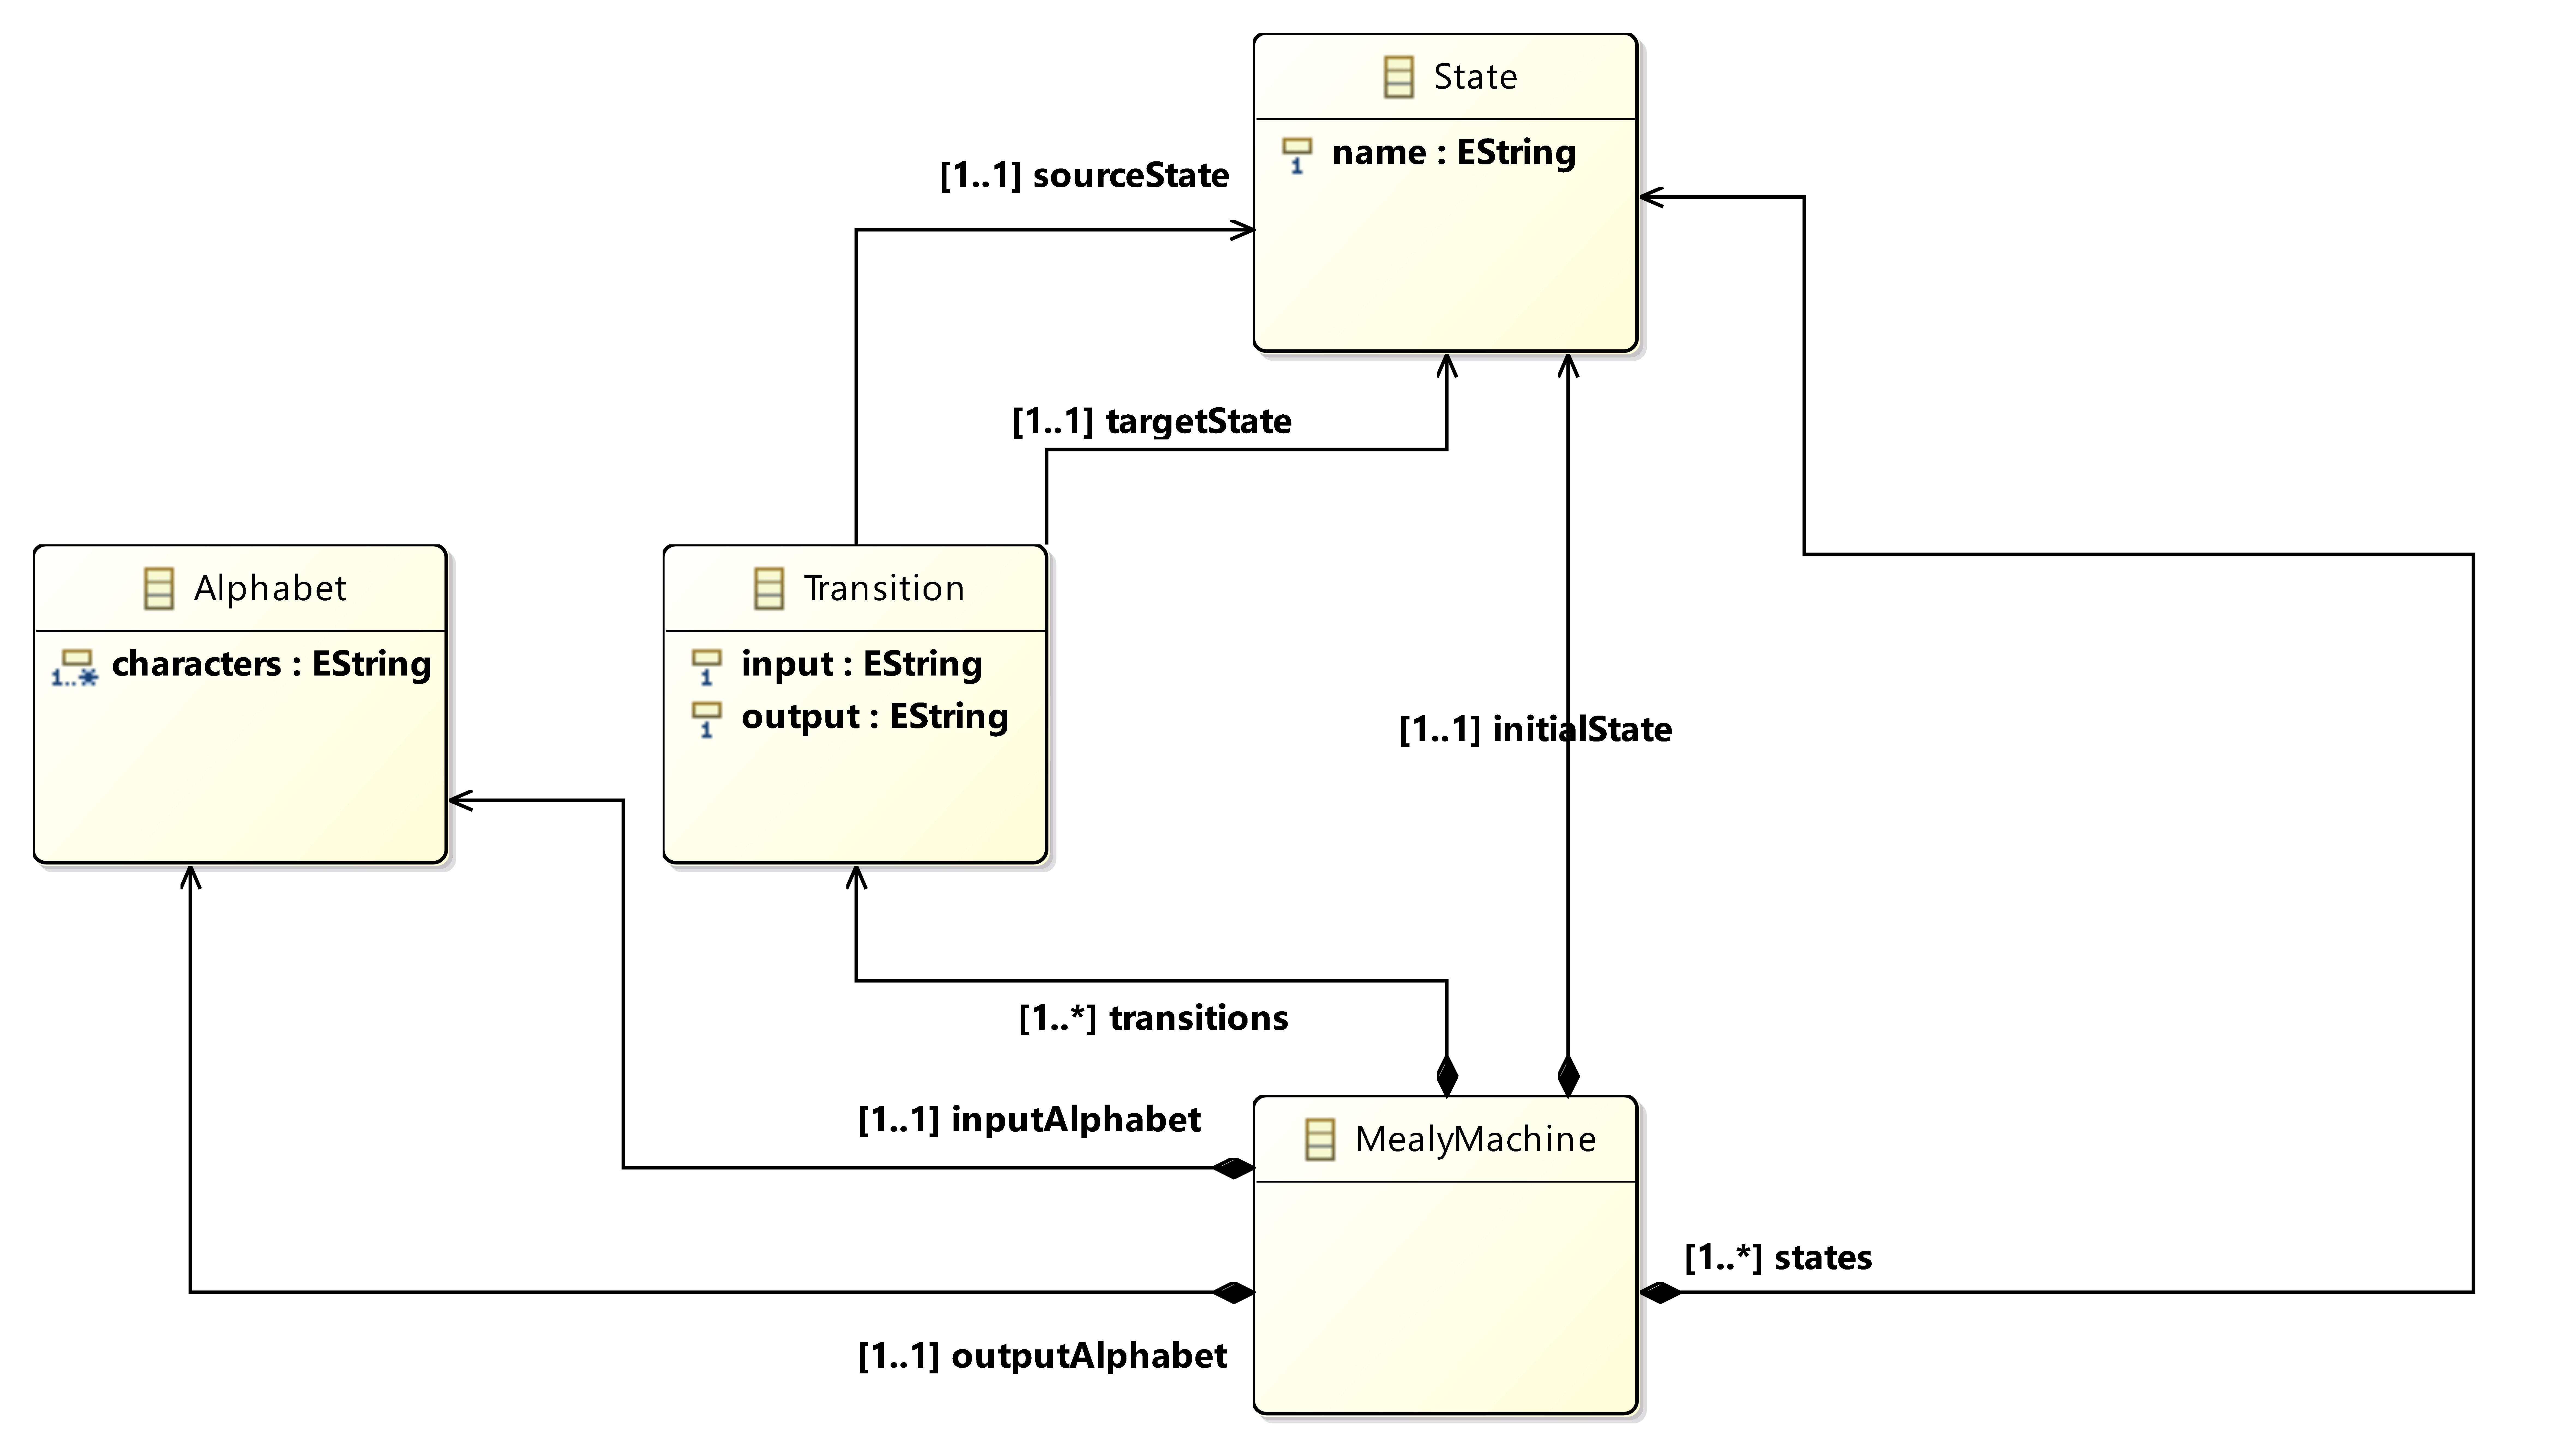
\includegraphics[width=130mm, keepaspectratio]{figures/appendix_mealymodel.jpg}
	}
	\caption{Ecore metamodel describing Mealy machines} 
	\label{fig_appendix_mealyecor}
\end{figure}

\begin{lstlisting}[caption=Xtext grammar describing Mealy machines.,label=li:appendix_xtext,float,floatplacement=H]
MealyMachine returns MealyMachine:
'MealyMachine'
'{'
'initialState' initialState=State
'states' '{' states+=State ( "," states+=State)* '}' 
'inputAlphabet' inputAlphabet=Alphabet
'outputAlphabet' outputAlphabet=Alphabet
'transitions' '{' transitions+=Transition ( "," transitions+=Transition)* '}' 
'}';

State returns State:
{State}
'State'
name=EString;

Alphabet returns Alphabet:
'Alphabet'
'{'
'characters' '{' characters+=EString ( "," characters+=EString)* '}' 
'}';

Transition returns Transition:
'Transition'
'{'
'input' input=EString
'output' output=EString
'sourceState' sourceState=[State|EString]
'targetState' targetState=[State|EString]
'}';

EString returns ecore::EString:
STRING | ID;
\end{lstlisting}

\begin{figure}[!ht] 
	\centering
	\fbox{
		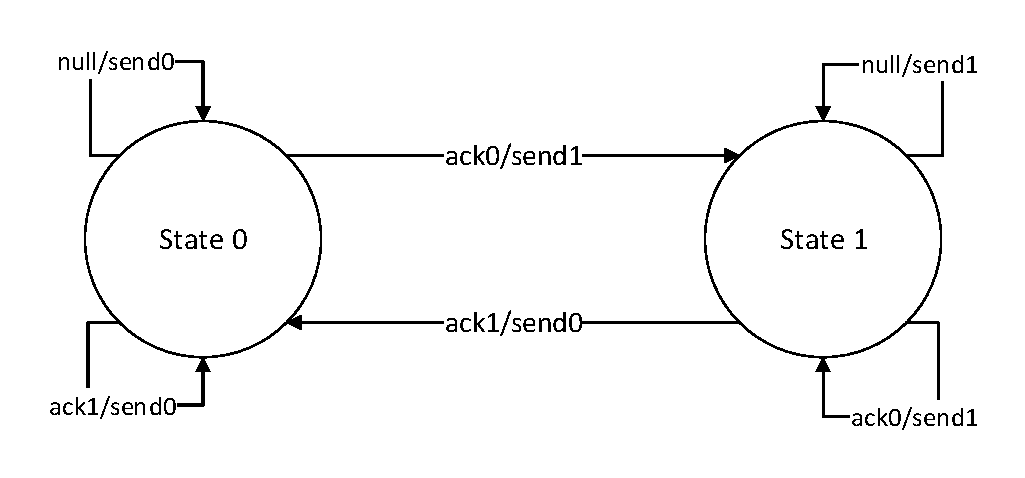
\includegraphics[width=130mm, keepaspectratio]{figures/alternatingbit.pdf}
	}
	\caption{Mealy machine describing the behavior of the alternating bit protocol} 
	\label{fig_alternatingbit}
\end{figure}

%----------------------------------------------------------------------------
\chapter{Pedestrian Crossing}
%----------------------------------------------------------------------------
\bigskip
\begin{lstlisting} [language=tex,caption=A possible run of the learning process,label=lst_examplelearning]
	Unknown output for input sequence: [control_toggle, control_interrupt]
	Ambiguous output: [trafficDisplay_blinkingYellow, trafficDisplay_red]
	Would you like to specify the output through an (I)O pair, an (L)TL expression, a (V)alid Trace or an I(N)valid Trace?
	>I
	Please provide the expected output:
	>TrafficDisplay.blinkingYellow
	
	Unknown output for input sequence: [control_toggle, control_interrupt, control_interrupt]
	Ambiguous output: [trafficDisplay_blinkingYellow, trafficDisplay_red]
	Would you like to specify the output through an (I)O pair, an (L)TL expression, a (V)alid Trace or an I(N)valid Trace?
	>I
	Please provide the expected output:
	>TrafficDisplay.red
	
	Unknown output for input sequence: [control_toggle, control_toggle, control_interrupt]
	Ambiguous output: [trafficDisplay_blinkingYellow, trafficDisplay_red]
	Would you like to specify the output through an (I)O pair, an (L)TL expression, a (V)alid Trace or an I(N)valid Trace?
	>I
	Please provide the expected output:
	>TrafficDisplay.blinkingYellow
	
	Unknown output for input sequence: [control_toggle, control_toggle, control_interrupt, control_interrupt]
	Ambiguous output: [trafficDisplay_blinkingYellow, trafficDisplay_red]
	Would you like to specify the output through an (I)O pair, an (L)TL expression, a (V)alid Trace or an I(N)valid Trace?
	>I
	Please provide the expected output:
	>TrafficDisplay.red
	
	Unknown output for input sequence: [control_toggle, control_toggle, control_toggle, control_interrupt]
	Ambiguous output: [trafficDisplay_blinkingYellow, trafficDisplay_red]
	Would you like to specify the output through an (I)O pair, an (L)TL expression, a (V)alid Trace or an I(N)valid Trace?
	>I
	Please provide the expected output:
	>TrafficDisplay.blinkingYellow
	
	Equivalence Query. Please provide a counterexamle:
	Control.interrupt Control.interrupt
	
	Unknown output for input sequence: [control_interrupt, control_interrupt, control_interrupt]
	Ambiguous output: [trafficDisplay_blinkingYellow, trafficDisplay_red]
	Would you like to specify the output through an (I)O pair, an (L)TL expression, a (V)alid Trace or an I(N)valid Trace?
	>V
	Please provide a valid trace:
	>Control.interrupt/TrafficDisplay.blinkingYellow Control.interrupt/TrafficDisplay.red Control.interrupt/TrafficDisplay.blinkingYellow Control.interrupt/TrafficDisplay.red
	
	Unknown output for input sequence: [control_interrupt, control_interrupt, control_toggle]
	Ambiguous output: [trafficDisplay_blinkingYellow, trafficDisplay_red, trafficDisplay_yellow, trafficDisplay_green]
	Would you like to specify the output through an (I)O pair, an (L)TL expression, a (V)alid Trace or an I(N)valid Trace?
	>I
	Please provide the expected output:
	>TrafficDisplay.green
	
	Unknown output for input sequence: [control_interrupt, control_toggle, control_interrupt]
	Ambiguous output: [trafficDisplay_blinkingYellow, trafficDisplay_red] 
	Would you like to specify the output through an (I)O pair, an (L)TL expression, a (V)alid Trace or an I(N)valid Trace?
	>I
	Please provide the expected output:
	>TrafficDisplay.red
	
	Equivalence Query. Please provide a counterexamle:
	>
\end{lstlisting}

\bigskip
\begin{figure}[!ht] 
	\centering
	\fbox{
		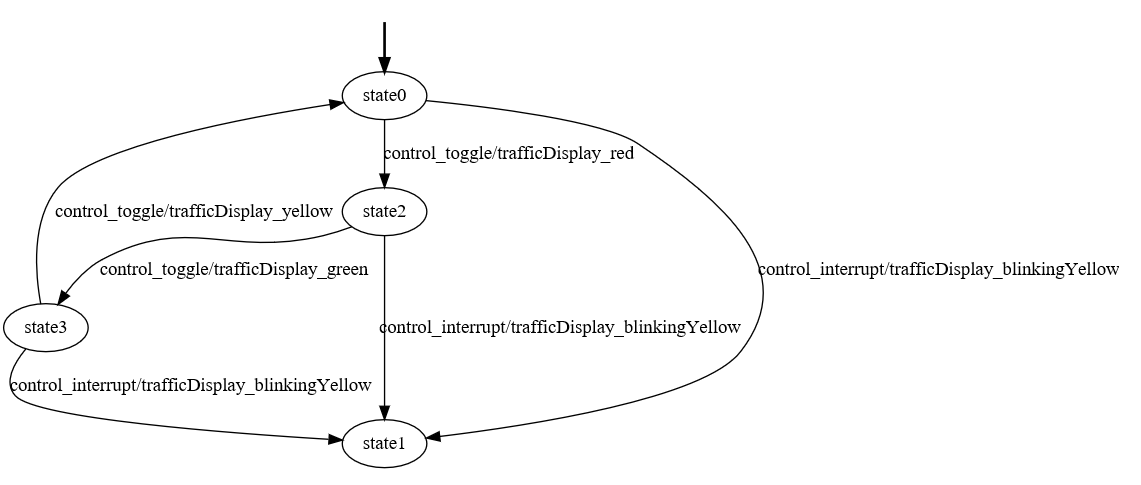
\includegraphics[width=130mm, keepaspectratio]{figures/casestudy_trafficlightinclomplete.PNG}
	}
	\caption{Equivalence query of the incomplete traffic light component} 
	\label{fig_trafficlightincomplete}
\end{figure}